\documentclass[16pt,a4paper]{article}
\usepackage[english]{babel}
\usepackage{hyperref}
\usepackage{graphicx}
\usepackage[margin=1in]{geometry}
\pagenumbering{gobble}
%\usepackage[T1]{fontenc}
%\usepackage{lmodern}
%\fontsize{size}{skip}
\title{\textbf{MoCA: Tool for Motif Conservation Analysis}}
\author{\underline{Saket Choudhary}, Anton Valouev}
\date{valouev@usc.edu}

\begin{document}
\maketitle
Motifs are short DNA sequences that appear recurrently and often have biological functions. They act as sequence specific binding sites for transcription factors. Motif analysis of ChIP-Seq datasets often reports multiple motifs. However, determining the quality of a reported motif is hard. Motifs reported by motif analysis tools such as MEME\cite{bailey2015meme} can often not be the 'true motifs' and  can have significant p-value(or E-values) for even 'false motifs'. 


Another metric often used to filter out motifs involves calculating the distance of the ChIP-seq peak with the center of the reported motif. This involves reporting the motifs appearing in $\pm$ 100 base pairs of the peak. 
However, with this approach will often not work for
identifying new co-transcription factor motifs.

%\begin{figure}
%	\centering
%	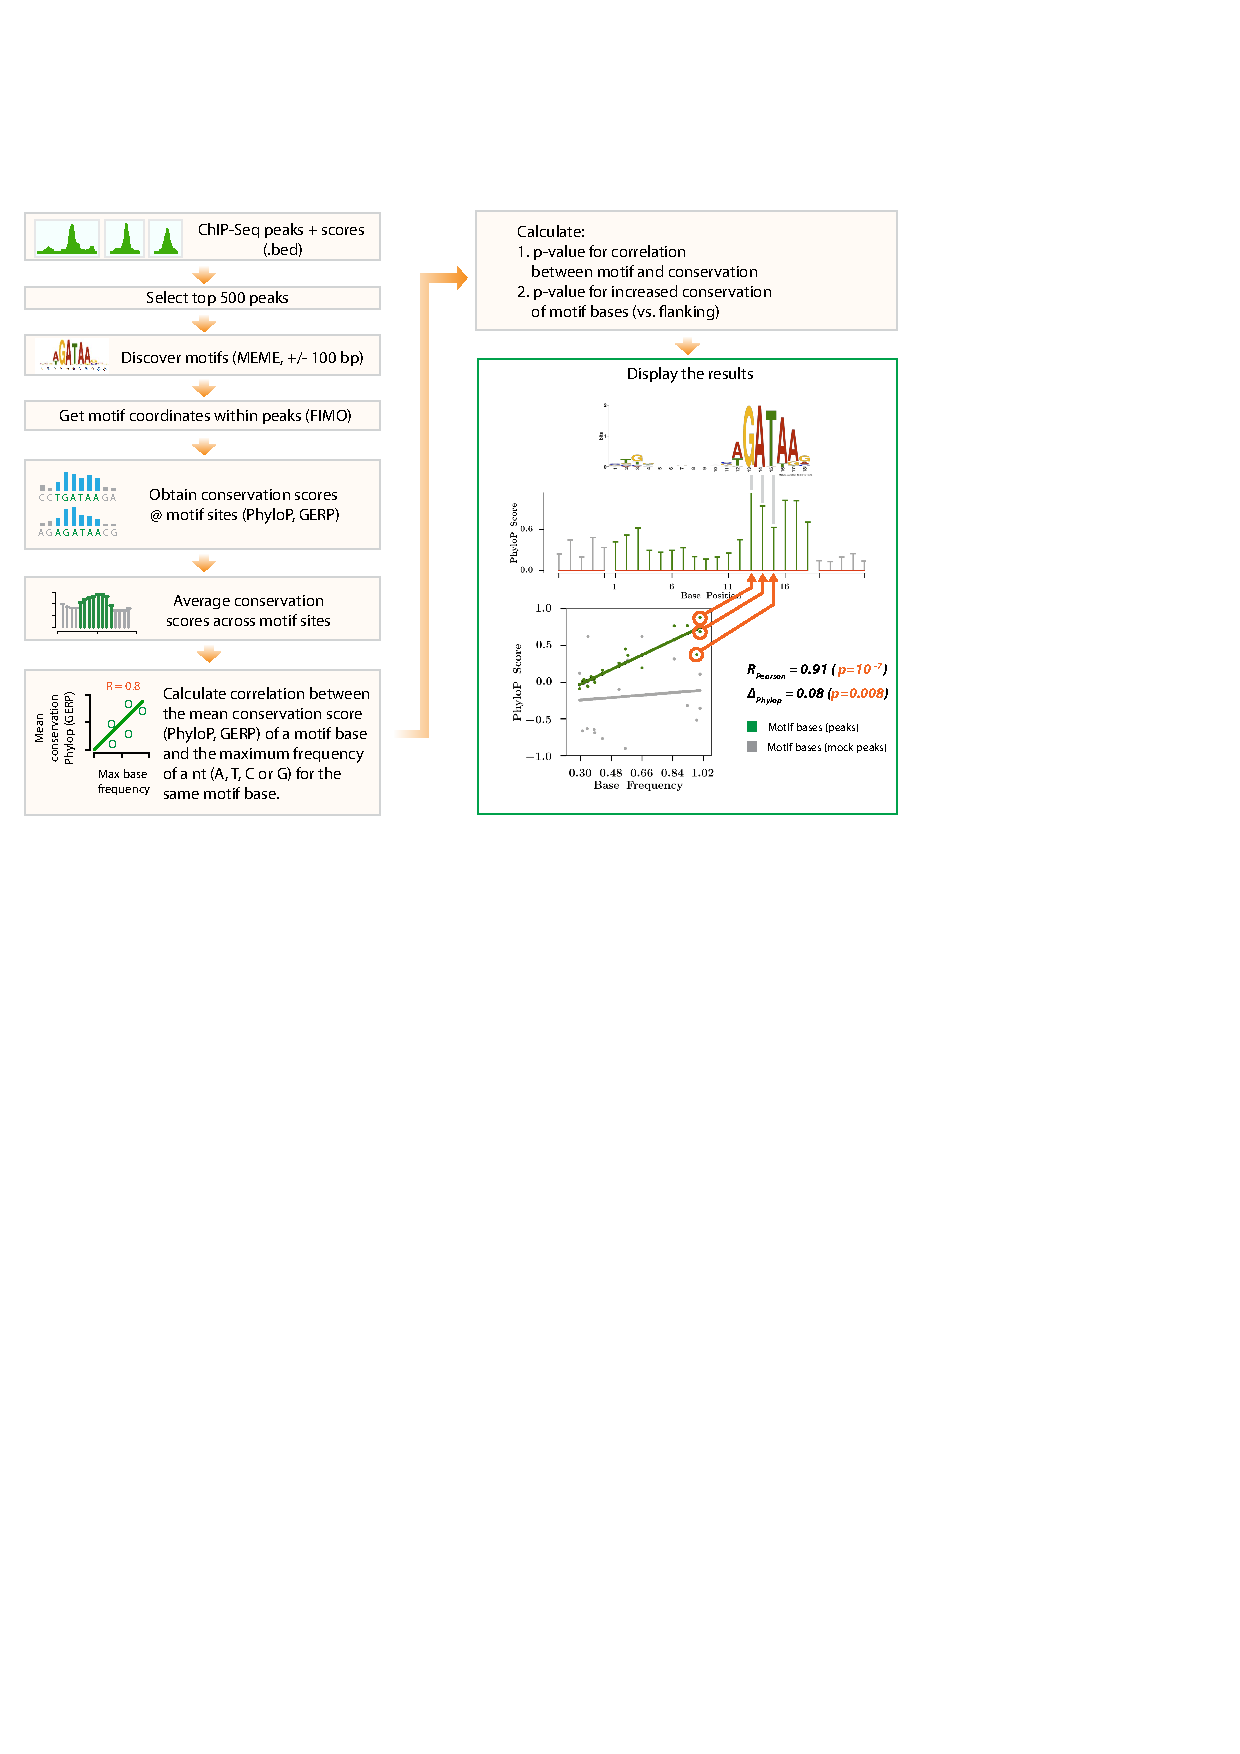
\includegraphics[scale=0.7]{workflow}
%	\caption {Workflow and conservation analysis plots generated by MoCA}
%\end{figure}

Any metric to assess the quality of motifs, should also rely on biological relevance besides the statistical analysis. 
Since the motif acts as a specific binding sequence, it can be expected to be conserved evolutionarily. We hence hypothesised that, a 'true motif' should exhibit high PhyloP\cite{siepel2006new} and Gerp\cite{davydov2010identifying} conservation scores.
In order to test the hypothesis, we developed MoCA, a tool to perform conservation analysis of reported motifs. MoCA makes use of the PhyloP and Gerp scores to assess the conservation profile of the motif bases and compares it with flanking bases and by searching for motifs in random genomic regions. If our hypothesis is true, the motif bases should show significantly more conservation as compared to the bases flanking the motifs on either side. 

We performed analysis on various ENCODE Chip-Seq datasets and found that the 'true motifs', validated experimentally do exhibit high conservation scores.

MoCA is available as a web service at \url{http://moca.usc.edu}
MoCA has an inbuilt support for directly analysing ENCODE Chip-Seq datasets, where the conservation analysis plots an be generated by specifying the ENCODE experiment id. 
\bibliographystyle{abbrv}
\bibliography{abstract}

\end{document}